\def\duedate{12/08/22}
\def\HWnum{5}
% Document setup
\documentclass[12pt]{article}
\usepackage[margin=1in]{geometry}
\usepackage{fancyhdr}
\usepackage{lastpage}

\pagestyle{fancy}
\lhead{Richard Whitehill}
\chead{PHYS 675 -- HW \HWnum}
\rhead{\duedate}
\cfoot{\thepage \hspace{1pt} of \pageref{LastPage}}

% Encoding
\usepackage[utf8]{inputenc}
\usepackage[T1]{fontenc}

% Math/Physics Packages
\usepackage{amsmath}
\usepackage{mathtools}
\usepackage[arrowdel]{physics}
\usepackage{siunitx}

\AtBeginDocument{\RenewCommandCopy\qty\SI}

% Reference Style
\usepackage{hyperref}
\hypersetup{
    colorlinks=true,
    linkcolor=blue,
    filecolor=magenta,
    urlcolor=cyan,
    citecolor=green
}

\newcommand{\eref}[1]{Eq.~(\ref{eq:#1})}
\newcommand{\erefs}[2]{Eqs.~(\ref{eq:#1})--(\ref{eq:#2})}

\newcommand{\fref}[1]{Fig.~\ref{fig:#1}}
\newcommand{\frefs}[2]{Figs.~\ref{fig:#1}--\ref{fig:#2}}

\newcommand{\tref}[1]{Table~\ref{tab:#1}}
\newcommand{\trefs}[2]{Tables~\ref{tab:#1}-\ref{tab:#2}}

% Figures and Tables 
\usepackage{graphicx}
\usepackage{float}
\usepackage{booktabs}

\newcommand{\bef}{\begin{figure}[h!]\begin{center}}
\newcommand{\eef}{\end{center}\end{figure}}

\newcommand{\bet}{\begin{table}[h!]\begin{center}}
\newcommand{\eet}{\end{center}\end{table}}

% tikz
\usepackage{tikz}
\usetikzlibrary{calc}
\usetikzlibrary{decorations.pathmorphing}
\usetikzlibrary{decorations.markings}
\usetikzlibrary{arrows.meta}
\usetikzlibrary{positioning}

% tcolorbox
\usepackage[most]{tcolorbox}
\usepackage{xcolor}
\usepackage{xifthen}
\usepackage{parskip}

\newcommand*{\eqbox}{\tcboxmath[
    enhanced,
    colback=black!10!white,
    colframe=black,
    sharp corners,
    size=fbox,
    boxsep=8pt,
    boxrule=1pt
]}

% Miscellaneous Definitions/Settings
\newcommand{\prob}[2]{\textbf{#1)} #2}

\setlength{\parskip}{\baselineskip}
\setlength{\parindent}{0pt}
\setlength{\headheight}{14.49998pt}
\addtolength{\topmargin}{-2.49998pt}


\begin{document}
    
\prob{16.4}{
Use the Bethe-Weizsa\"{a}cker relation to estimate the position in Fig. 16.2 of the $A = 127$ isobars with $Z = 48$, $49$, $67$, and $58$.
How would these isobars decay?
With what decay energies?
Estimate very crudely the lifetimes that you would expect.
}

We can write the mass excess in terms of the binding energy as
\begin{eqnarray}
    \Delta = -B + Zm_{H} + Nm_{n} - Auc^2
,\end{eqnarray}
where $m_{H} = 1.00784u$ and $m_{n} = 1.008665u$ with $u = \SI{931}{\MeV/c^2}$.
Additionally, the binding energy is given by the Bethe-Weis\"{a}cker relation
\begin{eqnarray}
    B = a_{v}A - a_{s}A^{2/3} - a_{\rm sym} \frac{(Z - N)^2}{A} - a_{c} Z^2 A^{-1/3}
,\end{eqnarray}
where $a_{v} = 15.6$, $a_{s} = 16.5$, $a_{\rm sym} = 23.3$, and $a_{c} = 0.72$ (in units of \SI{}{\MeV}).
Thus, we calculate the mass excesses for the $A = 127$ isobars with the $Z$ values above (and with $N = A - Z$) as $-62.2,\,-71.1,\,-72.2,\,68.8$ (again, in units of \SI{}{\MeV}).

For the decays, the minimum mass excess occurs for $Z = 53$, so for atoms with $Z < 53$ we may expect beta decay while for $Z > 53$ we may expect inverse beta decay.
The decay energies would just be the difference $\Delta|_{Z=53} - \Delta|_{Z \ne 53}$, which are given as $26.9,\,18.0,\,16.9,\,158.0$ \SI{}{\MeV}.
Using the Heisenberg uncertainty principle $\Delta E \Delta t \sim \hbar$ we can obtain a rough estimate of the lifetimes of these states to be $2.4 \times 10^{-23},\,3.7 \times 10^{-23},\,3.9 \times 10^{-23},\,4.2 \times 10^{-24}$ \SI{}{\s}.

\prob{16.5}{
Prepare a plot similar to Fig. 16.2 for the $A = 90$ isobars.
Show that \textit{two} parabolic curves appear.
Explain why.
How could the appearance of two such curves be introduced into the binding energy relation.
}

A plot of the mass excess data for $A = 90$ tabulated \href{https://wwwndc.jaea.go.jp/NuC/index.html}{here} is shown below:
\begin{center}
    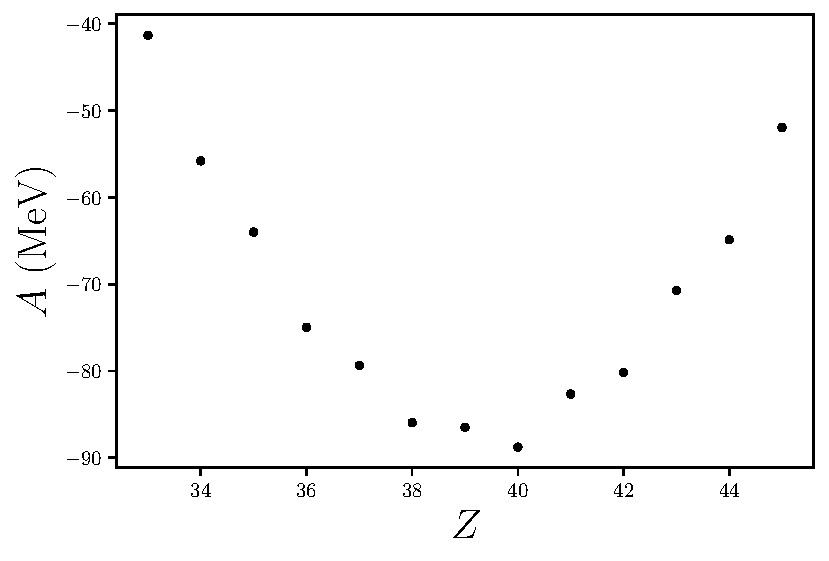
\includegraphics[width=0.6\textwidth]{prob6-5.pdf}
\end{center}
The two parabolas are very subtly separated, but the difference arises between even and odd $Z$ and $N$.
It seems that the difference is of a form
\begin{eqnarray}
    \delta B = \begin{cases}
        \phantom{-}\delta & Z~{\rm odd} \\
        -\delta & Z~{\rm even}
    .\end{cases}
\end{eqnarray}
Playing around with this correction term, it is found that $\delta$ between \SI{2}{\MeV} to \SI{3}{\MeV} reproduces the behavior quite well.
\begin{center}
    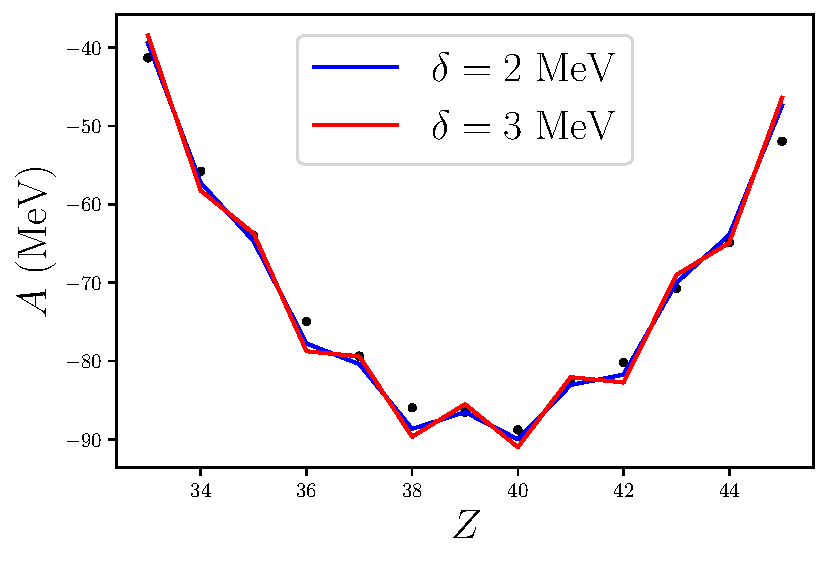
\includegraphics[width=0.6\textwidth]{prob6-5(1).pdf}
\end{center}

\prob{16.6}{
Consider possible decays $(A,Z) \rightarrow (A',Z')$.
Write down criteria that involve the corresponding atomic masses $m(A,Z)$ and that indicate when a nucleus $(A,Z)$ is stable against (a) alpha decay, (b) electron decay, (c) positron decay, and (d) electron capture.
}

The atomic mass is given by
\begin{eqnarray}
    m(A,Z) = Zm_{H} + Nm_{n} - \frac{B}{c^2}
,\end{eqnarray}
so the absolute mass difference after decay is
\begin{eqnarray}
    |m' - m| = |(Z' - Z)m_{H} + (N' - N)m_{n} - \frac{1}{c^2}(B(A',Z',N') - B(A,Z,N))|
.\end{eqnarray}
Clearly for alpha decay, we must have enough energy to produce the alpha particle.
That is,
\begin{eqnarray}
    m(A,Z) \geq m(A',Z') + m_{\alpha}
,\end{eqnarray}
where $m_{\alpha} = m(4,2)$.
The rest of the mass difference is the binding energy in the original configuration that does not go into the binding energy of the $\alpha$ particle or the new nuclide.
The other processes involve either protons or neutrons being produced or decaying while the mass number is held fixed.
In small atoms, it is favorable to have $Z \approx N$, so the processes where $Z \rightarrow Z \pm 1$ tend to make the nucleus more unstable, meaning that these nuclei tend to be stable against electron/positron decays and electron capture processes.
For larger atoms however, it is favorable to have an imbalance of neutrons and protons such that $N > Z$, so processes where $Z \rightarrow Z - 1$ tend to be more energetically favorable.
Thus larger atoms are expected to be more stable against electron decay processes. 

\prob{16.9}{
Verify that nucleons in the ground state of a nucleus indeed form a degenerate Fermi gas, i.e., occupy the lowest available levels, at all temperatures obtainable in the laboratory.
At what temperature (approximately) would a fair fraction of nucleons be excited?
}

The degenerate Fermi gas approximation is made at low temperatures.
That is $E_{F} \gg k_{B} T$, where $k_{B}$ is Boltzmann's constant.
For the processes we care about $E_{F} \approx \SI{40}{\MeV}$, which corresponds to temperatures $T \ll \SI{4.6e11}{\K}$, which is about 100,000 times hotter than a neutron star when formed.
The approximation we make that the nucleons are all in the lowest possible state would become poor when $T$ reaches an appreciable amount of $E_{F}/k_{B}$, which may be roughly 10\% of this value or \SI{5e10}{\K}.

\prob{16.11}{
Consider a nucleus with $A = 237$.
Use the semiempirical mass formula to:
}

a) Find $Z$ for the most stable isobar.

The semiempirical mass formula is given as
\begin{eqnarray}
    m = Zm_{p} + (A - Z)m_{n} - B/c^2
.\end{eqnarray}
We can calculate the $Z$ value for a fixed $A$ which is most stable as
\begin{eqnarray}
    c^2\dv{m}{Z} = (m_{p} - m_{n})c^2 - \dv{B}{Z} = a_{\rm sym} \frac{4(2Z - A)}{A} + 2a_{c} Z A^{-1/3} = 0
,\end{eqnarray}
assuming that $m_{p} \approx m_{n}$.
Solving for $Z$ in terms of $A$ and the paramaters $a_{\rm sym}$ and $a_{c}$ gives
\begin{eqnarray}
    Z_{\rm stable} = \frac{2A^{4/3}a_{\rm sym}}{4 A^{1/3}a_{\rm sym} + A a_{c}}
.\end{eqnarray}
Plugging in $A = 237$, we find $Z_{\rm stable} \approx 91$.


b) Discuss the stability of this nuclide for various likely decay modes.

This nuclide has a significantly larger number of nucleons than the most stable nuclide does, so the most likely form of decay is alpha decay by which the nuclide can shed 4 nucleons total.
Beta decay is also likely since this is a very large nucleus with a large number of neutrons, so the processes converting neutrons to protons is favorable.
The other processes involve the creation of neutrons at the expense of a proton, which are less favorable processes, so while they may occur, it is expected that they are suppressed.



\prob{16.13}{}

a) Consider isobars with $A$ odd.
How many stable isobars would you expect for a given value of $A$?
Why?

For small $A$, I would not expect many, if any, stable isobars since stability for small nuclei is achieved along the $Z = N$ line.
However, for larger $A$, I would expect several isobars with $N > Z$ to be stable, although at some point where $N \gg Z$, the isobars should be unstable because of the large imbalance between filled proton and neutron proton states.

b) Consider isobars with $N$ and $Z$ even.
Explain why more than one even stable isobar can occur.
Discuss an actual example.

From the perspective of filling states in the Fermi gas model potentials, it may be energetically favorable to have the 2 degenerate spin states at each level filled entirely in both the proton and neutron potential wells.
For example, the $^{120}_{52}{\rm Te}$ and $^{120}_{50}{\rm Sn}$ isobars are stable. 
Qualitatively, this can be interpreted as taking two particles from the neutron well and placing them in the proton well, which retains stability.


\end{document}
